\title{Buku Tugas Akhir ITS}
\author{Maulana, Alfi}

\documentclass[10pt,twoside]{report}
\usepackage[a5paper,top=25mm,left=25mm,right=20mm,bottom=25mm]{geometry}
\usepackage[singlespacing]{setspace}
\usepackage[indonesian]{babel}
\usepackage[pdfauthor={\@author},bookmarksnumbered,pdfborder={0 0 0}]{hyperref}
\usepackage[utf8]{inputenc}
\usepackage[table,xcdraw]{xcolor}
\usepackage[numbers]{natbib}
\usepackage{changepage}
\usepackage{enumitem}
\usepackage{eso-pic}
\usepackage{etoolbox}
\usepackage{graphicx}
\usepackage{lipsum}
\usepackage{lmodern}
\usepackage{longtable}
\usepackage{tabularx}
\usepackage{wrapfig}

\patchcmd{\cleardoublepage}{\hbox{}}{
  \thispagestyle{empty}
  \vspace*{\fill}
  \begin{center}\textit{[Halaman ini sengaja dikosongkan]}\end{center}
  \vfill}{}{}

\usepackage{fancyhdr}
\fancyhf{}
\renewcommand{\headrulewidth}{0pt}
\pagestyle{fancy}
\fancyfoot[CE,CO]{\thepage}
\patchcmd{\chapter}{plain}{fancy}{}{}
\patchcmd{\chapter}{empty}{plain}{}{}

\usepackage{titlesec}
\titleformat{\chapter}[display]{\bfseries\Large}{BAB \centering\Roman{chapter}}{0ex}{\vspace{0ex}\centering}
\titleformat{\section}{\bfseries\large}{\MakeUppercase{\thesection}}{1ex}{\vspace{1ex}}
\titleformat{\subsection}{\bfseries\large}{\MakeUppercase{\thesubsection}}{1ex}{}
\titleformat{\subsubsection}{\bfseries\large}{\MakeUppercase{\thesubsubsection}}{1ex}{}
\titlespacing{\chapter}{0ex}{0ex}{4ex}
\titlespacing{\section}{0ex}{1ex}{0ex}
\titlespacing{\subsection}{0ex}{0.5ex}{0ex}
\titlespacing{\subsubsection}{0ex}{0.5ex}{0ex}

\usepackage{listings}
\definecolor{comment}{RGB}{0,128,0}
\definecolor{string}{RGB}{255,0,0}
\definecolor{keyword}{RGB}{0,0,255}
\lstdefinestyle{codestyle}{
  commentstyle=\color{comment},
  stringstyle=\color{string},
  keywordstyle=\color{keyword},
  basicstyle=\footnotesize\ttfamily,
  numbers=left,
  numberstyle=\tiny,
  numbersep=5pt,
  frame=lines,
  breaklines=true,
  prebreak=\raisebox{0ex}[0ex][0ex]{\ensuremath{\hookleftarrow}},
  showstringspaces=false,
  upquote=true,
  tabsize=2,
}
\lstset{style=codestyle}

\begin{document}

  \AddToShipoutPictureBG*{
  \AtPageLowerLeft{
    \hspace{-3.5mm}
    \raisebox{0mm}{
      
\includegraphics[width=\paperwidth,height=\paperheight]{sampul/gambar/sampul-luar.png}
    }
  }
}

\thispagestyle{empty}

\newgeometry{
  top=95mm,
  left=25mm,
  right=20mm,
  bottom=25mm
}

\begin{flushleft}

  \sffamily
  \color{white}
  \fontseries{bx}
  \selectfont

  TUGAS AKHIR - EC184801

\vspace{6ex}

\begin{large}
  PENGEMBANGAN LINGKUNGAN SIMULASI UNTUK PENGUJIAN \emph{SOCIALLY ASSISTIVE ROBOTS} MENGGUNAKAN ROS 2 DAN GAZEBO
\end{large}

\vspace{4ex}

Muhammad Alfi Maulana Fikri \\
NRP 0721 17 4000 0009

\vspace{2ex}

Dosen Pembimbing \\
Prof. Dr. Ir. Mauridhi Hery Purnomo, M.Eng. \\
Dr. I Ketut Eddy Purnama, S.T., M.T.

\vspace{6ex}

DEPARTEMEN TEKNIK KOMPUTER \\
Fakultas Teknologi Elektro dan Informatika Cerdas \\
Institut Teknologi Sepuluh Nopember \\
Surabaya 2021


\end{flushleft}

\restoregeometry


  \AddToShipoutPictureBG*{
  \AtPageLowerLeft{
    % Ubah nilai berikut jika posisi horizontal background tidak sesuai
    \hspace{-3.5mm}

    % Ubah nilai berikut jika posisi vertikal background tidak sesuai
    \raisebox{0mm}{
      
\includegraphics[width=\paperwidth,height=\paperheight]{sampul/gambar/sampul-dalam.png}
    }
  }
}

% Menyembunyikan nomor halaman
\thispagestyle{empty}

% Pengaturan margin untuk menyesuaikan konten sampul
\newgeometry{
  top=95mm,
  left=25mm,
  right=20mm,
  bottom=25mm
}

\begin{flushleft}

  % Pemilihan font sans serif
  \sffamily

  % Pemilihan font bold
  \fontseries{bx}
  \selectfont

  TUGAS AKHIR - EC184801

\vspace{6ex}

\begin{large}
  PENGEMBANGAN LINGKUNGAN SIMULASI UNTUK PENGUJIAN \emph{SOCIALLY ASSISTIVE ROBOTS} MENGGUNAKAN ROS 2 DAN GAZEBO
\end{large}

\vspace{4ex}

Muhammad Alfi Maulana Fikri \\
NRP 0721 17 4000 0009

\vspace{2ex}

Dosen Pembimbing \\
Prof. Dr. Ir. Mauridhi Hery Purnomo, M.Eng. \\
Dr. I Ketut Eddy Purnama, S.T., M.T.

\vspace{6ex}

DEPARTEMEN TEKNIK KOMPUTER \\
Fakultas Teknologi Elektro dan Informatika Cerdas \\
Institut Teknologi Sepuluh Nopember \\
Surabaya 2021


\end{flushleft}

\restoregeometry

  \cleardoublepage

  \setlength{\parindent}{2em}
  \setlength{\parskip}{1ex}

  \begin{center}
  \large
  \textbf{PERNYATAAN KEASLIAN\\TUGAS AKHIR}
\end{center}

\thispagestyle{empty}
\vspace{2ex}

Dengan ini saya menyatakan bahwa isi buku Tugas Akhir dengan judul
``\textbf{Pengembangan Lingkungan Simulasi untuk Pengujian \emph{Socially Assistive Robots} Menggunakan ROS 2 dan Gazebo}''
adalah benar hasil karya intelektual mandiri, diselesaikan tanpa menggunakan bahan-bahan yang tidak diijinkan dan bukan merupakan karya pihak lain yang saya akui sebagai karya sendiri.

Semua referensi yang dikutip maupun dirujuk telah ditulis secara lengkap pada daftar pustaka.
Apabila ternyata pernyataan ini tidak benar, saya bersedia menerima sanksi sesuai peraturan yang berlaku.

\vspace{4ex}

\begin{flushright}
  \begin{tabular}[b]{c}
    Surabaya, Juni 2021\\
    \\
    \\
    \\
    \\
    Muhammad Alfi Maulana Fikri\\
    0721 17 4000 0009
  \end{tabular}
\end{flushright}

  \cleardoublepage

  \begin{center}
	\large
  \textbf{LEMBAR PENGESAHAN}
\end{center}

\thispagestyle{empty}

\begin{center}
  \small

  \textbf{PENGEMBANGAN LINGKUNGAN SIMULASI UNTUK PENGUJIAN \emph{SOCIALLY ASSISTIVE ROBOTS} MENGGUNAKAN ROS 2 DAN GAZEBO}
\end{center}

\begingroup
  \small

  \begin{center}
    Tugas Akhir ini disusun untuk memenuhi salah satu syarat memperoleh gelar Sarjana Teknik di Institut Teknologi Sepuluh Nopember Surabaya
  \end{center}

  \begin{center}
    Oleh: Muhammad Alfi Maulana Fikri (NRP. 0721 17 4000 0009)
  \end{center}

  \begingroup
    \setlength{\tabcolsep}{0pt}
    \noindent
    \begin{tabularx}{\textwidth}{X r}
    Tanggal Ujian : 23 Juli 2021 & Periode Wisuda : September 2021
    \end{tabularx}
  \endgroup

  \begin{center}
    Disetujui Oleh:
  \end{center}

  \begingroup
    \setlength{\tabcolsep}{0pt}
    \noindent
    \begin{tabularx}{\textwidth}{X c}
      Prof. Dr. Ir. Mauridhi Hery Purnomo, M.Eng. & (Pembimbing I) \\
      NIP. 19580916 198601 1 001                  & \\
      & \\
      & \\
      Dr. I Ketut Eddy Purnama, S.T., M.T.        & (Pembimbing II) \\
      NIP. 19690730 199512 1 001                  & \\
      & \\
      & \\
      Mochamad Hariadi, ST., M.Sc., Ph.D.         & (Penguji I) \\
      NIP. 19691209 199703 1 002                  & \\
      & \\
      & \\
      Dr. Supeno Mardi Susiki Nugroho, S.T., M.T. & (Penguji II) \\
      NIP. 19700313 199512 1 001                  & \\
    \end{tabularx}
  \endgroup

  \vspace{4ex}

  \begin{center}
    Mengetahui, \\
    Kepala Departemen Teknik Komputer \\

    \vspace{8ex}

    \underline{Dr. Supeno Mardi Susiki Nugroho, S.T., M.T.} \\
    NIP. 19700313 199512 1 001
  \end{center}
\endgroup

  \cleardoublepage

  \pagenumbering{roman}

  \begin{center}
  \large\textbf{ABSTRAK}
\end{center}

\vspace{2ex}

\begingroup
  \setlength{\tabcolsep}{0pt}
  \noindent
  \begin{tabularx}{\textwidth}{l >{\centering}m{2em} X}
    Nama        &:& Muhammad Alfi Maulana Fikri \\
    Judul       &:&	Pengembangan Lingkungan Simulasi untuk Pengujian \emph{Socially Assistive Robots} Menggunakan ROS 2 dan Gazebo \\
    Pembimbing  &:& 1. Prof. Dr. Ir. Mauridhi Hery Purnomo, M.Eng. \\
                & & 2. Dr. I Ketut Eddy Purnama, S.T., M.T. \\
  \end{tabularx}
\endgroup

Selama beberapa tahun terakhir,
  robot telah mengalami perkembangan yang cukup signifikan.
Salah satu bentuk perkembangan tersebut adalah \emph{socially assistive robots} (SARs) yang mampu memberikan bantuan kepada pengguna dalam bentuk interaksi sosial.
Namun, karena sifatnya yang melibatkan interaksi langsung dengan pengguna,
  pengujian pada SARs akan menjadi sulit dan beresiko.
Untuk itu, pada penelitian ini kami mengajukan lingkungan simulasi untuk pengujian SARs yang dibuat menggunakan simulator Gazebo.
% Di dalam lingkungan simulasi ini,
%   model robot akan diujikan dengan model pengguna serta model-model objek lain secara virtual.
Agar pengujian yang dilakukan di simulasi bisa diterapkan pada robot fisik,
  sistem kontroler yang ada pada robot akan dibuat secara terabstraksi dengan memisah setiap komponen menjadi \emph{nodes} menggunakan ROS 2.
% Dengan adanya abstraksi tersebut,
%   program utama robot dapat digunakan pada berbagai sistem yang ada,
%   terlepas dari sistem itu ada di simulasi maupun ada pada robot fisik.
Hasilnya,
  lingkungan simulasi yang dibuat dapat digunakan untuk melakukan pengujian SARs secara virtual.
selain itu, ketika diujikan pada robot fisik,
  tindakan yang dihasilkan memiliki kesamaan dengan yang dihasilkan oleh model robot di simulasi.

Kata Kunci: Simulasi, \emph{Assistive Robotics}, ROS2, Gazebo.

  \cleardoublepage

  \begin{center}
  \large\textbf{ABSTRACT}
\end{center}

\vspace{2ex}

\begingroup
  \setlength{\tabcolsep}{0pt}
  \noindent
  \begin{tabularx}{\textwidth}{l >{\centering}m{2em} X}
    \emph{Name}     &:& Muhammad Alfi Maulana Fikri \\
    \emph{Title}    &:&	\emph{Development of Simulation Environment for Socially Assistive Robots Testing Using ROS 2 and Gazebo} \\
    \emph{Advisors} &:& 1. Prof. Dr. Ir. Mauridhi Hery Purnomo, M.Eng. \\
                    & & 2. Dr. I Ketut Eddy Purnama, S.T., M.T. \\
  \end{tabularx}
\endgroup

\emph{
  Over the past few years,
    robots have undergone significant developments.
  One of this development is socially assistive robots (SARs) which are able to assist users in the form of social interaction.
  However, due to their nature which involves direct interaction with the user,
    testing SARs could be difficult and risky.
  For this reason, in this study we propose a simulation environment for testing SARs created using the Gazebo simulator.
  In order for the test performed in the simulation could be applied to real robots,
    the controller system in the robot will be abstracted by separating each component into nodes using ROS 2.
  As a result, the created simulation environment could be used to test SARs virtually.
    In addition, when tested on a real robot,
    the resulting actions are similar to those generated by the robot model in the simulation.
}

\emph{Keywords}: \emph{Simulation}, \emph{Assistive Robotics}, ROS 2, Gazebo.

  \cleardoublepage

  \begin{center}
  \Large
  \textbf{KATA PENGANTAR}
\end{center}

\vspace{2ex}

Puji dan syukur kehadirat Allah SWT atas segala limpahan berkah, rahmat, serta hidayah-Nya, penulis  dapat menyelesaikan penelitian ini dengan judul
``\textbf{Pengembangan Lingkungan Simulasi untuk Pengujian \emph{Socially Assistive Robots} Menggunakan ROS 2 dan Gazebo}''.
Penelitian ini disusun dalam rangka pemenuhan bidang riset di Departemen Teknik Komputer,
  serta digunakan sebagai persyaratan menyelesaikan pendidikan S1.

Dalam penyusunan buku ini,
  penulis mengucapkan terima kasih kepada Keluarga yang telah memberikan dorongan spiritual dan material dalam penyelesaian penelitian ini.
Terutama kepada Ayah atas didikannya kepada penulis selama ini,
  semoga beliau husnul khatimah di sana, aamiin.

Penulis juga mengucapkan terima kasih kepada Bapak Prof. Dr. Ir. Mauridhi Hery Purnomo, M.Eng.,
  Bapak Dr. I Ketut Eddy Purnama, S.T., M.T.,
  dan Bapak Muhtadin ST., MT. atas arahan dan bimbingan selama pengerjaan penelitian tugas akhir ini.
Serta kepada Bapak-ibu dosen pengajar Departemen Teknik Komputer atas pengajaran dan perhatian yang diberikan kepada penulis selama ini.

Dan terakhir,
  terima kasih kepada rekan-rekan ICHIRO ITS, Robotika ITS, dan B201 crew atas pengalamannya kepada penulis.
Serta kepada rekan-rekan seperjuangan Teknik Komputer 2017, E57, dan penghuni rumah anak TK.

Kesempurnaan hanya milik Allah SWT, untuk itu penulis memohon segenap kritik dan saran yang  membangun.
Semoga penelitian ini dapat memberikan manfaat bagi kita semua, aamiin.

\begin{flushright}
  \begin{tabular}[b]{c}
    Surabaya, Juli 2021\\
    \\
    \\
    \\
    \\
    Muhammad Alfi Maulana Fikri
  \end{tabular}
\end{flushright}

  \cleardoublepage

  \renewcommand*\contentsname{DAFTAR ISI}
  \addcontentsline{toc}{chapter}{\contentsname}
  \tableofcontents
  \cleardoublepage

  \renewcommand*\listfigurename{DAFTAR GAMBAR}
  \addcontentsline{toc}{chapter}{\listfigurename}
  \listoffigures
  \cleardoublepage

  \renewcommand*\listtablename{DAFTAR TABEL}
  \addcontentsline{toc}{chapter}{\listtablename}
  \listoftables
  \cleardoublepage

  \pagenumbering{arabic}

  \chapter{PENDAHULUAN}
\label{chap:pendahuluan}

% Ubah bagian-bagian berikut dengan isi dari pendahuluan

Penelitian ini dilatarbelakangi oleh \lipsum[1][1-5]

\section{Latar Belakang}
\label{sec:latarbelakang}

Pesatnya perkembangan roket yang merupakan \lipsum[1]

\lipsum[2]

\section{Permasalahan}
\label{sec:permasalahan}

Dari permasalahan tersebut maka \lipsum[1][1-6]

\section{Tujuan}
\label{sec:Tujuan}

Tujuan dari \lipsum[1][1-3] adalah:

\begin{enumerate}[nolistsep]

  \item Membuat \lipsum[2][1-3]

  \item \lipsum[3][1-3]

\end{enumerate}

\section{Batasan Masalah}
\label{sec:batasanmasalah}

Batasan-batasan dari \lipsum[1][1-3] adalah:

\begin{enumerate}[nolistsep]

  \item Mempermudah \lipsum[2][1-3]

  \item \lipsum[3][1-5]

  \item \lipsum[4][1-5]

\end{enumerate}

\section{Sistematika Penulisan}
\label{sec:sistematikapenulisan}

Laporan penelitian tugas akhir ini terbagi menjadi \lipsum[1][1-3] yaitu:

\begin{enumerate}[nolistsep]

  \item \textbf{BAB I Pendahuluan}

  Bab ini berisi \lipsum[2][1-5]

  \vspace{2ex}

  \item \textbf{BAB II Tinjauan Pustaka}

  Bab ini berisi \lipsum[3][1-5]

  \vspace{2ex}

  \item \textbf{BAB III Desain dan Implementasi Sistem}

  Bab ini berisi \lipsum[4][1-5]

  \vspace{2ex}

  \item \textbf{BAB IV Pengujian dan Analisa}

  Bab ini berisi \lipsum[5][1-5]

  \vspace{2ex}

  \item \textbf{BAB V Penutup}

  Bab ini berisi \lipsum[6][1-5]

\end{enumerate}

  \cleardoublepage

  \chapter{TINJAUAN PUSTAKA}
\label{chap:tinjauanpustaka}

Pada bab ini akan dijelaskan teori-teori penunjang yang digunakan sebagai bahan acuan dan referensi untuk penelitian yang dilakukan.
Teori-teori yang dijelaskan pada bab ini akan dipaparkan dalam urutan yang sistematis,
  dimulai dari hal paling mendasar yang digunakan pada penelitian ini seperti penjelasan mengenai \emph{assistive robotics}, Gazebo, dan ROS,
  hingga penjelasan lebih dalam yang berhubungan dengan sistem yang dibuat dan pengujian yang dilakukan seperti Kinect dan SLAM.

\subimport{2-tinjauan-pustaka}{1-assistive-robotics.tex}
\subimport{2-tinjauan-pustaka}{2-ros2.tex}
\subimport{2-tinjauan-pustaka}{3-gazebo.tex}
\subimport{2-tinjauan-pustaka}{4-holonomic-robot.tex}
\subimport{2-tinjauan-pustaka}{5-imu.tex}
\subimport{2-tinjauan-pustaka}{6-posture-device.tex}
\subimport{2-tinjauan-pustaka}{7-depth-camera.tex}
% \subimport{2-tinjauan-pustaka}{8-mediapipe.tex}
% \subimport{2-tinjauan-pustaka}{9-slam.tex}

  \cleardoublepage

  \chapter{DESAIN DAN IMPLEMENTASI}
\label{chap:desainimplementasi}

Pada bab ini akan diuraikan desain dan implementasi dari sistem yang telah dibuat.
Seperti yang terlihat pada gambar \ref{fig:blogdiagramkerja},
  desain dan implementasi yang akan diuraikan ini dimulai dari pengembangan model robot dan pengguna yang dibuat sebagai file dengan bentuk SDFormat.
Pengembangan kemudian akan dilakukan untuk lingkungan simulasi yang terdiri dari sebuah lingkungan \emph{outdoor} dan lingkungan \emph{indoor}.

\begin{figure}[ht]
  \centering
  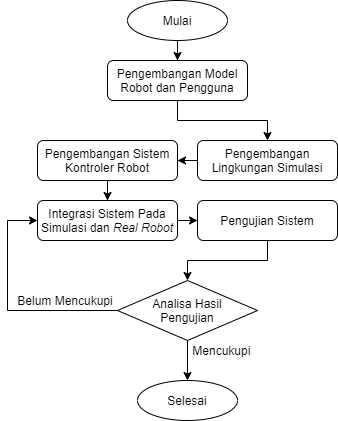
\includegraphics[scale=0.6]{gambar/blok-diagram-kerja.png}
  \caption{Blok diagram dari alur pekerjaan.}
  \label{fig:blogdiagramkerja}
\end{figure}

Kemudian, sistem robot berbasis ROS 2 akan dikembangkan.
Pengembangan sistem tersebut dilakukan secara terabstraksi yang mana nantinya akan terpisah menjadi 3 bagian,
  dimana sistem yang mengatur komponen yang ada di simulasi akan dibentuk sebagai \emph{Gazebo Plugins},
  sistem yang mengatur komponen yang ada di \emph{real robot} akan dibentuk sebagai \emph{controller node},
  dan terakhir sistem yang mengatur tindakan robot secara umum untuk simulasi dan \emph{real robot} akan dibentuk sebagai \emph{behavior node}.

Bagian akhir dari pekerjaan ini adalah pengujian untuk sistem yang telah dibuat.
Pengujian nantinya akan terdiri dari beberapa bagian yang menguji berbagai aspek yang ada pada sistem yang telah dikembangkan.
Jika hasil pengujian dirasa belum mencukupi, integrasi sistem pada simulasi dan \emph{real robot} akan dilakukan kembali hingga hasil pengujian di keduanya cukup sesuai.
Bagian ini secara lebih lanjut akan dijelaskan pada bab \ref{chap:hasilpengujian}.

\subimport{3-desain-implementasi}{1-model-robot.tex}
\subimport{3-desain-implementasi}{2-model-pengguna.tex}
\subimport{3-desain-implementasi}{3-lingkungan-simulasi.tex}
\subimport{3-desain-implementasi}{4-behavior-node.tex}
\subimport{3-desain-implementasi}{5-integrasi-plugin.tex}
\subimport{3-desain-implementasi}{6-integrasi-robot.tex}

  \cleardoublepage

  \chapter{PENGUJIAN DAN ANALISIS}
\label{chap:pengujiananalisis}

% Ubah bagian-bagian berikut dengan isi dari pengujian dan analisis

Pada penelitian ini dipaparkan \lipsum[1][1-5]

\section{Skenario Pengujian}
\label{sec:skenariopengujian}

Pengujian dilakukan dengan \lipsum[1-2]

\section{Evaluasi Pengujian}
\label{sec:analisispengujian}

Dari pengujian yang \lipsum[1]

% Contoh pembuatan tabel
\begin{longtable}{|c|c|c|}
  \caption{Hasil Pengukuran Energi dan Kecepatan}
  \label{tb:EnergiKecepatan}\\
  \hline
  \rowcolor[HTML]{C0C0C0}
  \textbf{Energi} & \textbf{Jarak Tempuh} & \textbf{Kecepatan} \\
  \hline
  10 J & 1000 M & 200 M/s \\
  20 J & 2000 M & 400 M/s \\
  30 J & 4000 M & 800 M/s \\
  40 J & 8000 M & 1600 M/s \\
  \hline
\end{longtable}

\lipsum[2-4]

  \cleardoublepage

  \chapter{PENUTUP}
\label{chap:penutup}

% Ubah bagian-bagian berikut dengan isi dari penutup

\section{Kesimpulan}
\label{sec:kesimpulan}

Berdasarkan hasil pengujian yang \lipsum[1][1-3] sebagai berikut:

\begin{enumerate}[nolistsep]

  \item Pembuatan \lipsum[2][1-3]

  \item \lipsum[2][4-6]

  \item \lipsum[2][7-10]

\end{enumerate}

\section{Saran}
\label{chap:saran}

Untuk pengembangan lebih lanjut pada \lipsum[1][1-3] antara lain:

\begin{enumerate}[nolistsep]

  \item Memperbaiki \lipsum[2][1-3]

  \item \lipsum[2][4-6]

  \item \lipsum[2][7-10]

\end{enumerate}

  \cleardoublepage

  \renewcommand\bibname{DAFTAR PUSTAKA}
  \addcontentsline{toc}{chapter}{\bibname}
  \bibliographystyle{unsrtnat}
  \bibliography{pustaka/pustaka.bib}
  \cleardoublepage

  \begin{center}
  \Large
  \textbf{BIOGRAFI PENULIS}
\end{center}

\addcontentsline{toc}{chapter}{BIOGRAFI PENULIS}

\vspace{2ex}

\begin{wrapfigure}{L}{0.3\textwidth}
  \centering
  \vspace{-3ex}
  % Ubah file gambar berikut dengan file foto dari mahasiswa
  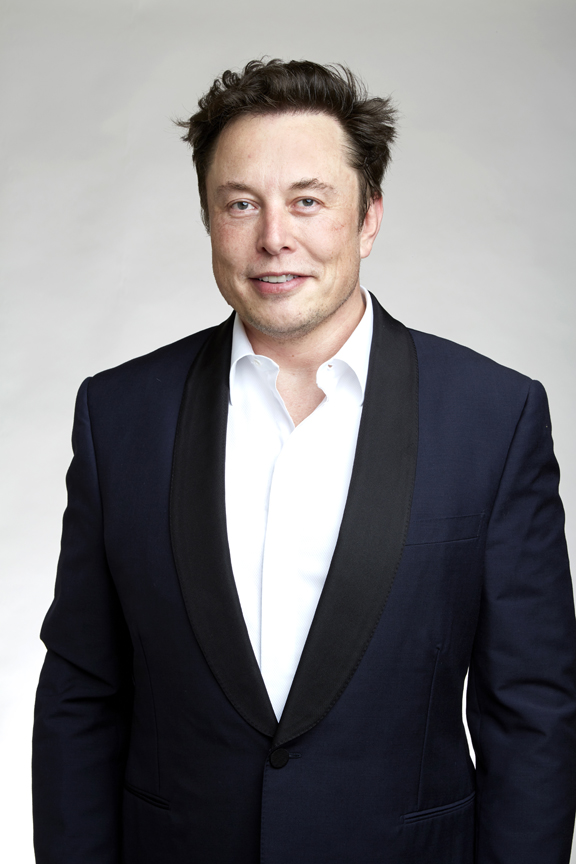
\includegraphics[width=0.3\textwidth]{gambar/elon.jpg}
  \vspace{-4ex}
\end{wrapfigure}

% Ubah kalimat berikut dengan biografi dari mahasiswa
Elon Reeve Musk, lahir pada \lipsum[1]

\lipsum[2]

  \cleardoublepage

\end{document}
